\newcommand{\ww}{0.32333} 
\begin{figure}[H] 
    \captionsetup[subfloat]{justification=raggedright,singlelinecheck=false, position=bottom,labelformat=empty} % 
    \subfloat[Wielkość obrazu O1: 500x512]{
       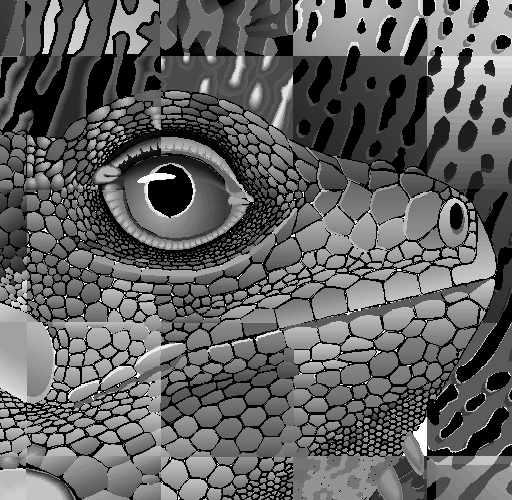
\includegraphics[width=\ww\linewidth]{../zad2/img3/I1.png}}  \hfill% 
    \subfloat[Wielkość obrazu Id: 500x512\\ PSNR = 15.7643]{
       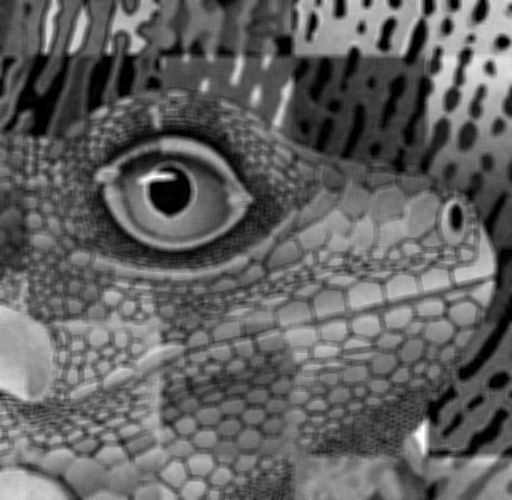
\includegraphics[width=\ww\linewidth]{../zad2/img3/I3.png}}  \hfill% 
    \subfloat[Wielkość obrazu I: 500x512]{
       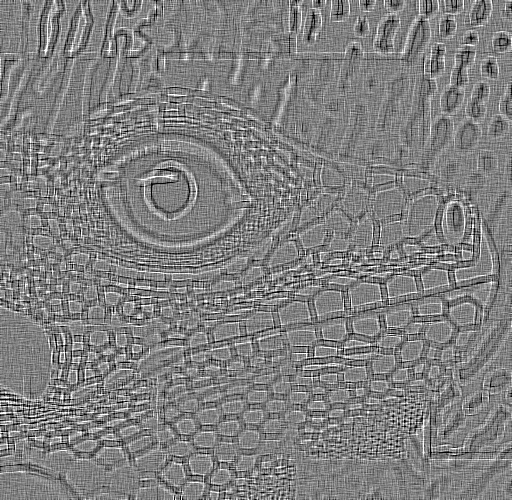
\includegraphics[width=\ww\linewidth]{../zad2/img3/I5.png}}  \\ 
    \subfloat[Os = O + szum\\ PSNR = 19.9894]{
       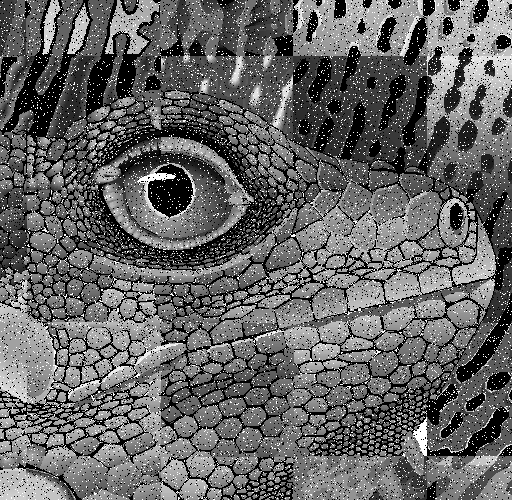
\includegraphics[width=\ww\linewidth]{../zad2/img3/I2.png}}  \hfill% 
    \subfloat[O - Id]{
       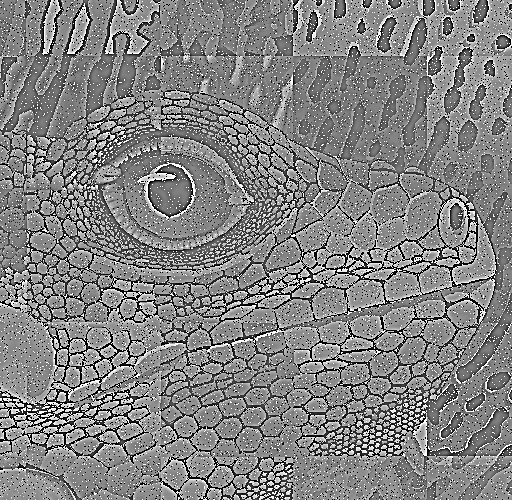
\includegraphics[width=\ww\linewidth]{../zad2/img3/I4.png}}  \hfill% 
    \subfloat[O - I\\ PSNR = 17.1441]{
       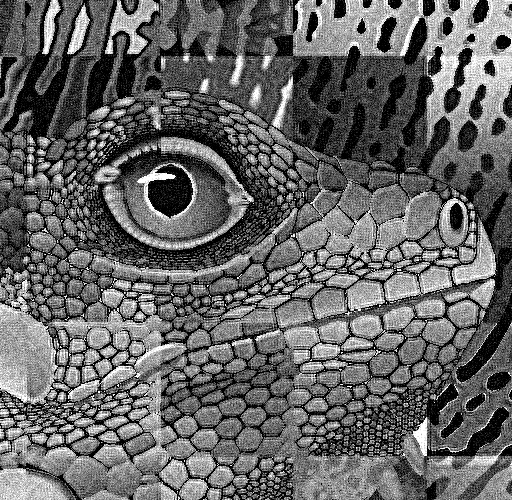
\includegraphics[width=\ww\linewidth]{../zad2/img3/I6.png}}
\caption{Porownanie}  
\label{fig:../zad2/result_3.tex} 
\end{figure} 
\let\ww\undefined 
maski użyte do filtracji obrazu:
$$
Md = \begin{bmatrix}
2.0^{-2} & 2.0^{-2} & 2.0^{-2} & 2.0^{-2} & 2.0^{-2} & 2.0^{-2} & 2.0^{-2} \\ 
2.0^{-2} & 2.0^{-2} & 2.0^{-2} & 2.0^{-2} & 2.0^{-2} & 2.0^{-2} & 2.0^{-2} \\ 
2.0^{-2} & 2.0^{-2} & 2.0^{-2} & 2.0^{-2} & 2.0^{-2} & 2.0^{-2} & 2.0^{-2} \\ 
2.0^{-2} & 2.0^{-2} & 2.0^{-2} & 2.0^{-2} & 2.0^{-2} & 2.0^{-2} & 2.0^{-2} \\ 
2.0^{-2} & 2.0^{-2} & 2.0^{-2} & 2.0^{-2} & 2.0^{-2} & 2.0^{-2} & 2.0^{-2} \\ 
2.0^{-2} & 2.0^{-2} & 2.0^{-2} & 2.0^{-2} & 2.0^{-2} & 2.0^{-2} & 2.0^{-2} \\ 
2.0^{-2} & 2.0^{-2} & 2.0^{-2} & 2.0^{-2} & 2.0^{-2} & 2.0^{-2} & 2.0^{-2}
\end{bmatrix}
$$
 \\ 
$$
Mg = \begin{bmatrix}
-1.0^{0} & -1.0^{0} & -1.0^{0} \\ 
-1.0^{0} & 8.0^{0} & -1.0^{0} \\ 
-1.0^{0} & -1.0^{0} & -1.0^{0}
\end{bmatrix}
$$